\documentclass[12pt]{article}
\usepackage[brazil]{babel}
\usepackage[a4paper, total={6.5in, 9.5in}]{geometry}
\usepackage[utf8]{inputenc}

\usepackage{authblk}
\usepackage{lipsum}
\usepackage{xcolor}
\usepackage{listings}
\usepackage[normalem]{ulem}
\usepackage{amssymb}
\usepackage{float}
\usepackage{graphicx}
\usepackage{amsmath}
\usepackage{amsthm}
\usepackage{amssymb}
\usepackage{verbatimbox}
\newtheorem{theorem}{Theorem}[section]
\newtheorem{lemma}[theorem]{Lemma}

\definecolor{codegreen}{rgb}{0,0.6,0}
\definecolor{codegray}{rgb}{0.5,0.5,0.5}
\definecolor{codered}{rgb}{0.8,0,0}
\definecolor{backcolour}{rgb}{0.95,0.95,0.92}

\usepackage{inconsolata}
\lstset{
    language=python,
    backgroundcolor=\color{backcolour},   
    commentstyle=\color{codegreen},
    keywordstyle=\color{blue},
    numberstyle=\tiny\color{codegray},
    stringstyle=\color{codered},
    basicstyle=\ttfamily\small,
    numberstyle=\footnotesize,
    numbers=left,
    backgroundcolor=\color{white},
    frame=single,
    tabsize=2,
    rulecolor=\color{white},
    title=\lstname,
    escapeinside={\%*}{*)},
    breaklines=true,
    breakatwhitespace=true,
    framextopmargin=2pt,
    framexbottommargin=2pt,
    inputencoding=utf8,
    extendedchars=true,
    showstringspaces=false,
    literate={á}{{\'a}}1 {ã}{{\~a}}1 {é}{{\'e}}1 {Ó}{{\'O}}1 {Ã}{{\~A}}1 {í}{{\'i}}1 {ó}{{\'o}}1 {ç}{{\.c}}1 {ê}{{\^e}}1 {ú}{{\'u}}1,
}

% \pagecolor[rgb]{0.1,0.1,0.1} %black
% \color[rgb]{0.75,0.75,0.75} %grey

\title{\textbf{Segurança Computacional\\ \Large{Advanced Encryption Standard}}}
\author{Pedro Henrique de Brito Agnes, 18/0026305 \\
Pedro Pessoa Ramos, 18/0026488}
\affil{Dep. Ciência da Computação - Universidade de Brasília (UnB) \vspace{-2ex}}
\date{}

\begin{document}
\maketitle

\section{Implementação do AES}
A implementação do AES foi feita fixa para a versão de 128 bits e para isso foi criado o arquivo \texttt{aes.py} na pasta \texttt{src} usando a linguagem python preferencialmente na versão 3.6 ou acima. Para executar o programa para cifrar o arquivo \texttt{sample/dupla.ppm}, por exemplo com uma chave pseudo-aleatória usando o padrão de \textit{rounds} no modo ECB e salvar o criptograma no arquivo \texttt{sample/10r.ppm}, deve ser usado o seguinte comando:

\begin{lstlisting}
python src/aes.py sample/dupla.ppm -o sample/10r.ppm
\end{lstlisting}

O primeiro argumento que o programa recebe é o arquivo que contém a mensagem. Logo em seguida, está sendo passado o argumento \texttt{-o}, que é obrigatório e representa o arquivo onde será impresso o criptograma. Como não foi passada uma chave pré-existente, será gerada a chave durante a execução e ela será salva na pasta \texttt{keys} e será impressa uma mensagem informando o nome exato do arquivo que a contém. Existem outros argumentos opcionais que podem ser listados com o \texttt{-h}:

\begin{lstlisting}
python src/aes.py -h
\end{lstlisting}

Segue a lista de argumentos aceitos:
\begin{itemize}
    \item \textbf{-k} - Arquivo com a chave para criptografar/descriptografar. Argumento obrigatório se for acionada a opção para descriptografar.
    \item \textbf{-o} - Arquivo onde será feito o output. Obrigatório.
    \item \textbf{-r} - Número positivo que representa a quantidade de \textit{rounds} que o AES irá usar. Se não passado um valor, será usado o padrão de 10.
    \item \textbf{-d} - Argumento que indica que o programa vai descriptografar. Deve ser passado no final do comando sem parâmetros adicionais.
    \item \textbf{-m} - Modo de operação do AES. Opções disponíveis são ECB ou CTR. Se não passado um valor, será usado o modo ECB.
    \item \textbf{-n} - Número inicial para o modo CTR (nonce). Se não passado, será usado como 0.
\end{itemize}

Portanto, como exemplo, para cifrar o mesmo arquivo do exemplo acima usando a mesma chave (ex.: \texttt{keys/key\_1}) com 1 \textit{round} e colocando o output no arquivo \texttt{sample/1r.ppm}, pode ser usado o seguinte comando:

\begin{lstlisting}
python src/aes.py sample/dupla.ppm -k keys/key_1 -r 1 -o sample/1r.ppm
\end{lstlisting}

Da mesma forma, para decifrá-lo no arquivo \texttt{sample/decoded.ppm} por exemplo, pode-se usar o comando abaixo:

\begin{lstlisting}
python src/aes.py sample/1r.ppm -k keys/key_1 -r 1 -o sample/decoded.ppm -d
\end{lstlisting}

\subsection{Aspectos Técnicos}
O AES é uma cifra de blocos, portanto, o seu funcionamento pode ser descrito pelo seguinte diagrama considerando o modo ECB:

\begin{figure}[H]
	\centering
    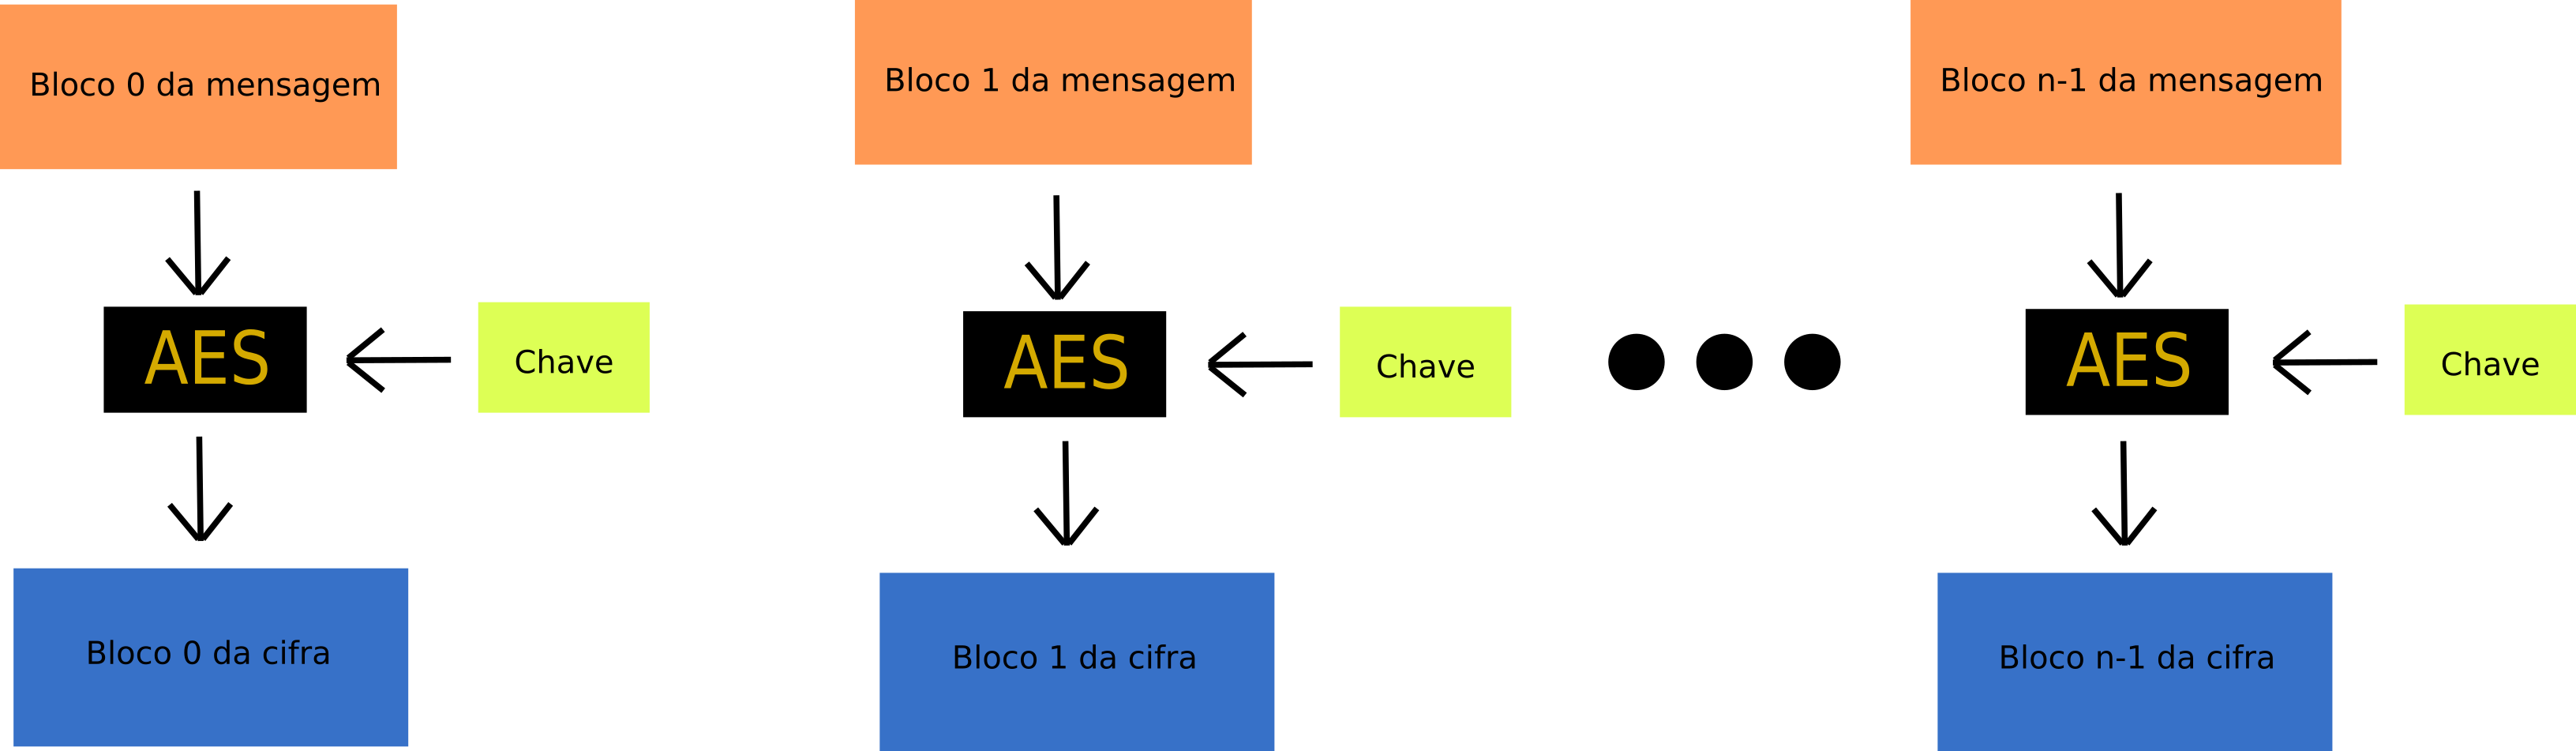
\includegraphics[width=\textwidth]{img/ecb.png}
    \caption{Cifra de bloco no modo ECB}
\end{figure}

Para a implementação descrita na seção anterior, temos 2 arquivos principais que realizam as operações do AES, ambos na pasta \texttt{src/symmetric}. O \texttt{cipher} é usado para cifrar e o \texttt{decipher} é usado para decifrar. De forma resumida, o funcionamento da cifração se dá na seguinte forma:

\begin{lstlisting}
self.addRoundKey()          # realiza o XOR com a chave inicial
for i in range(rounds):     # itera sobre os rounds
    self.expandKey(i)       # transforma a chave
    self.subBytes()
    self.shiftRows()
    if i != rounds-1:       # não realiza o mixColumns no último round
        self.mixColumns()
    
    self.addRoundKey()      # Realiza o XOR com a chave da rodada
\end{lstlisting}

Já para a decifração, é feito o contrário das operações, sendo que algumas foram modificadas apesar de ter o mesmo nome e segue a seguinte rotina:

\begin{lstlisting}
for x in range(rounds):     # vai até a chave final obtida na cifração
    self.expandKey(x)

for i in range(rounds):     # itera sobre os rounds
    self.addRoundKey()      # realiza o XOR com a chave da rodada
    if i != 0:              # não realiza o mixColumns no round inicial
        self.mixColumns()

    self.shiftRows()
    self.subBytes()
    self.shrinkKey(rounds-1-i) # operação reversa da expandKey
    
self.addRoundKey()          # Realiza o XOR com a chave inicial
\end{lstlisting}

A chave é obrigatoriamente de 16 bytes de tamanho e pode ser obtida pelo arquivo passado por parâmetro ou gerada automaticamente por um número randômico. Se passada uma chave inválida ao programa, uma mensagem de erro será exibida. Todas as funções relacionadas à chave podem ser encontradas em \texttt{src/util/passphrase.py}

\subsubsection{Processamento da Mensagem em Blocos}
Esta etapa é a primeira a ser executada ao obter o arquivo com a mensagem e, portanto, os blocos são obtidos de simples segmentos contínuos de 16 bytes da mensagem até chegar ao final. Para o caso do tamanho da mensagem não ser divisível por 16, são acrescentados caracteres representados pelo ASCII 7B em hexadecimal ao final para completar, que ficará apenas no último bloco. Conforme especificação, os blocos, ao serem transformados em matrizes 4x4, são colocados verticalmente na matriz. Consideremos o seguinte array:

\begin{center}
\addvbuffer[12pt 8pt]{\begin{tabular}{|cccccccccccccccc|}
    1 & 2 & 3 & 4 & 5 & 6 & 7 & 8 & 9 & 10 & 11 & 12 & 13 & 14 & 15 & 16
\end{tabular}}
\end{center}

O bloco gerado por ele será o seguinte:

\begin{center}
\addvbuffer[12pt 8pt]{\begin{tabular}{|cccc|}
    1 & 5 & 9 & 13\\
    2 & 6 & 10 & 14\\
    3 & 7 & 11 & 15\\
    4 & 8 & 12 & 16
\end{tabular}}
\end{center}

\subsubsection{addRoundKey}
Na cifração, esta é a primeira etapa que é realizada no primeiro round duas vezes, uma no início ainda com a chave inicial e outra no final, após alterar a chave com o \texttt{expandKey}. Nos rounds seguintes, a etapa é realizada apenas 1 vez, sendo o último passo. Consiste de apenas um XOR realizado entre um byte do bloco com um byte da chave, sendo feita a operação entre os elementos de mesmo \textit{index}. Na decifração é feito o contrário, portanto dos primeiro round até o round $n-1$, é feito o XOR normalmente com a chave da rodada ao início dela e no último round é executado mais uma vez no final de tudo com a chave que terá retornado à original.

\subsubsection{expandKey}
É a função usada na cifração que modifica a chave a cada rodada. Esta começa realizando um XOR entre a primeira coluna da chave e a última coluna com um shift realizado nos elementos e alterada pela mesma tabela usada no \texttt{subBytes}. Em seguida, com o resultado deste XOR é feito mais um XOR do primeiro elemento com o valor da tabela RCON de acordo com o round atual e o resultado deste será a primeira coluna da chave modificada. Já para as 3 demais colunas, é feito o XOR entre a coluna original da chave e a coluna anterior da nova chave, sendo uma operação de natureza cumulativa. A operação é sempre realizada em cima da chave já modificada pelo \texttt{expandKey} anterior, o que garante que sempre será usada uma chave diferente em cada rodada.

Foi criada uma função para a decifração que reverte o \texttt{expandKey} chamada \texttt{shrinkKey}. Como ela é usada para reverter a operação, é feito exatamente o inverso da anterior.

\subsubsection{subBytes}
Esta operação é executada em cada round e, basicamente utiliza uma tabela para a substituição do byte por um outro valor de acordo com o index representado pelo byte atual. A tabela é chamada de \texttt{s\_box} e pode ser vista abaixo:

\noindent
\addvbuffer[12pt 8pt]{\begin{tabular}{|c|c|c|c|c|c|c|c|c|c|c|c|c|c|c|c|}
    \hline
    99 & 124 & 119 & 123 & 242 & 107 & 111 & 197 &  48 &   1 & 103 &  43 & 254 & 215 & 171 & 118 \\
    \hline
    202 & 130 & 201 & 125 & 250 &  89 &  71 & 240 & 173 & 212 & 162 & 175 & 156 & 164 & 114 & 192 \\
    \hline
    183 & 253 & 147 &  38 &  54 &  63 & 247 & 204 &  52 & 165 & 229 & 241 & 113 & 216 &  49 &  21 \\
    \hline
    4 & 199 &  35 & 195 &  24 & 150 &   5 & 154 &   7 &  18 & 128 & 226 & 235 &  39 & 178 & 117 \\
    \hline
    9 & 131 &  44 &  26 &  27 & 110 &  90 & 160 &  82 &  59 & 214 & 179 &  41 & 227 &  47 & 132 \\
    \hline
    83 & 209 &   0 & 237 &  32 & 252 & 177 &  91 & 106 & 203 & 190 &  57 &  74 &  76 &  88 & 207 \\
    \hline
    208 & 239 & 170 & 251 &  67 &  77 &  51 & 133 &  69 & 249 &   2 & 127 &  80 &  60 & 159 & 168 \\
    \hline
    81 & 163 &  64 & 143 & 146 & 157 &  56 & 245 & 188 & 182 & 218 &  33 &  16 & 255 & 243 & 210 \\
    \hline
    205 &  12 &  19 & 236 &  95 & 151 &  68 &  23 & 196 & 167 & 126 &  61 & 100 &  93 &  25 & 115 \\
    \hline
    96 & 129 &  79 & 220 &  34 &  42 & 144 & 136 &  70 & 238 & 184 &  20 & 222 &  94 &  11 & 219 \\
    \hline
    224 &  50 &  58 &  10 &  73 &   6 &  36 &  92 & 194 & 211 & 172 &  98 & 145 & 149 & 228 & 121 \\
    \hline
    231 & 200 &  55 & 109 & 141 & 213 &  78 & 169 & 108 &  86 & 244 & 234 & 101 & 122 & 174 &   8 \\
    \hline
    186 & 120 &  37 &  46 &  28 & 166 & 180 & 198 & 232 & 221 & 116 &  31 &  75 & 189 & 139 & 138 \\
    \hline
    112 &  62 & 181 & 102 &  72 &   3 & 246 &  14 &  97 &  53 &  87 & 185 & 134 & 193 &  29 & 158 \\
    \hline
    225 & 248 & 152 &  17 & 105 & 217 & 142 & 148 & 155 &  30 & 135 & 233 & 206 &  85 &  40 & 223 \\
    \hline
    140 & 161 & 137 &  13 & 191 & 230 &  66 & 104 &  65 & 153 &  45 &  15 & 176 &  84 & 187 &  22 \\
    \hline
\end{tabular}}

A tabela acima pode ser revertida pela tabela mostrada abaixo, chamada \texttt{s\_box\_inv}:

\noindent
\addvbuffer[12pt 8pt]{\begin{tabular}{|c|c|c|c|c|c|c|c|c|c|c|c|c|c|c|c|}
    \hline
    82 &   9 & 106 & 213 &  48 &  54 & 165 &  56 & 191 &  64 & 163 & 158 & 129 & 243 & 215 & 251 \\
    \hline
    124 & 227 &  57 & 130 & 155 &  47 & 255 & 135 &  52 & 142 &  67 &  68 & 196 & 222 & 233 & 203 \\
    \hline
    84 & 123 & 148 &  50 & 166 & 194 &  35 &  61 & 238 &  76 & 149 &  11 &  66 & 250 & 195 &  78 \\
    \hline
    8 &  46 & 161 & 102 &  40 & 217 &  36 & 178 & 118 &  91 & 162 &  73 & 109 & 139 & 209 &  37 \\
    \hline
    114 & 248 & 246 & 100 & 134 & 104 & 152 &  22 & 212 & 164 &  92 & 204 &  93 & 101 & 182 & 146 \\
    \hline
    108 & 112 &  72 &  80 & 253 & 237 & 185 & 218 &  94 &  21 &  70 &  87 & 167 & 141 & 157 & 132 \\
    \hline
    144 & 216 & 171 &   0 & 140 & 188 & 211 &  10 & 247 & 228 &  88 &   5 & 184 & 179 &  69 &   6 \\
    \hline
    208 &  44 &  30 & 143 & 202 &  63 &  15 &   2 & 193 & 175 & 189 &   3 &   1 &  19 & 138 & 107 \\
    \hline
    58 & 145 &  17 &  65 &  79 & 103 & 220 & 234 & 151 & 242 & 207 & 206 & 240 & 180 & 230 & 115 \\
    \hline
    150 & 172 & 116 &  34 & 231 & 173 &  53 & 133 & 226 & 249 &  55 & 232 &  28 & 117 & 223 & 110 \\
    \hline
    71 & 241 &  26 & 113 &  29 &  41 & 197 & 137 & 111 & 183 &  98 &  14 & 170 &  24 & 190 &  27 \\
    \hline
    252 &  86 &  62 &  75 & 198 & 210 & 121 &  32 & 154 & 219 & 192 & 254 & 120 & 205 &  90 & 244 \\
    \hline
    31 & 221 & 168 &  51 & 136 &   7 & 199 &  49 & 177 &  18 &  16 &  89 &  39 & 128 & 236 &  95 \\
    \hline
    96 &  81 & 127 & 169 &  25 & 181 &  74 &  13 &  45 & 229 & 122 & 159 & 147 & 201 & 156 & 239 \\
    \hline
    160 & 224 &  59 &  77 & 174 &  42 & 245 & 176 & 200 & 235 & 187 &  60 & 131 &  83 & 153 &  97 \\
    \hline
    23 &  43 &   4 & 126 & 186 & 119 & 214 &  38 & 225 & 105 &  20 &  99 &  85 &  33 &  12 & 125 \\
    \hline
\end{tabular}}

\subsubsection{shiftRows}
A etapa é executada a cada round e passa em cada uma das 4 linhas do bloco da mensagem e mantém a primeira inalterada, a segunda é feito um \textit{shift} dos bytes para a direita, como se um byte empurrase o outro uma casa para a esquerda. Na linha seguinte, os bytes são deslocados 2 casas à esquerda e na última linha, 3 casas. A etapa descrita acima é para a cifragem. Para a decifragem, os bytes são deslocados à direita para inverter a operação.

\subsubsection{mixColumns}
A etapa é executada em todos os rounds com exceção do último no caso da cifragem, enquanto na decifragem a operação é excluída do primeiro round a fim de fazer o contrário para decifrar. A operação realiza uma multiplicação de cada coluna do bloco com uma matriz fixa, trocando as operações de soma por XOR e a multiplicação é feita em um campo finito $GF(8)$. Segue a matriz usada abaixo:

\begin{center}
\addvbuffer[12pt 8pt]{\begin{tabular}{|cccc|}
    2 & 3 & 1 & 1\\
    1 & 2 & 3 & 1\\
    1 & 1 & 2 & 3\\
    3 & 1 & 1 & 2
\end{tabular}}
\end{center}

Para a inversão da operação, apenas é trocada a matriz para a descrita abaixo:

\begin{center}
\addvbuffer[12pt 8pt]{\begin{tabular}{|cccc|}
    14 & 11 & 13 & 9\\
    9 & 14 & 11 & 13\\
    13 & 9 & 14 & 11\\
    11 & 13 & 9 & 14
\end{tabular}}
\end{center}

\section{Modo CTR}

Para a implementação do modo CTR, foram usadas as mesmas classes python que no ECB e para a utilização dele, 2 novos parâmetros podem ser passados para o programa conforme descrito na seçãoanterior. Portanto, se o usuário deseja cifrar o arquivo \texttt{sample/dupla.ppm} no modo CTR com o \texttt{nonce} 0 produzindo o output no arquivo \texttt{sample/ctr.ppm} com o restantes dos parâmetros padrões, pode-se usar o seguinte comando:

\begin{lstlisting}
python src/aes.py sample/dupla.ppm -o sample/ctr.ppm -m ctr
\end{lstlisting}

O \texttt{nonce} pode ser modificado com o parâmetro \texttt{-n}, assim como os todos os parâmetros informados na seção anterior. Como exemplo, pode-se cifrar o mesmo arquivo no modo CTR com a chave \texttt{keys/key\_2}, o valor do \texttt{nonce} 123456789 e nove rodadas, produzindo o output em \texttt{sample/r9ctr.ppm} com o seguinte comando:

\begin{lstlisting}
python src/aes.py sample/dupla.ppm -o sample/r9ctr.ppm -k keys/key_2 -r 9 -m ctr -n 123456789
\end{lstlisting}

Para decifrar o CTR, não é necessária a utilização do \texttt{-d}, basta "cifrar a cifra" novamente que o resultado será a mensagem original. Mas para isso, deve ser usada além da mesma chave, o mesmo \texttt{nonce} como mostrado no comando abaixo:

\begin{lstlisting}
python src/aes.py sample/r9ctr.ppm -o sample/decoded_ctr.ppm -k keys/key_2 -r 9 -m ctr -n 123456789
\end{lstlisting}

\subsection{Aspectos Técnicos}

O CTR é o modo de cifra de blocos que implementa um contador e nele existem diferenças consideráveis em relação ao ECB. Na implementação feita do CTR, o que é passado para o algoritmo de cifragem no lugar da mensagem é um bloco gerado a partir do \texttt{nonce} somado ao contador que tem o valor de seu index. A quantidade de blocos gerados deve ser a mesma quantidade dos blocos gerados pela mensagem e cada bloco é montado pelos bytes obtidos do número de 128 bits gerado pela operação.

tudo o que foi descrito acima, tirando a parte da decifragem foi reutilizado, pois o processo do AES em si se mantém inalterado. Adicionalmente, em relação ao ECB, foram criados if's adicionais e uma nova função para gerar os blocos a partir do \texttt{nonce} com o contador. O processo do ECB pode ser descrito pela imagem abaixo:

\begin{figure}[H]
	\centering
    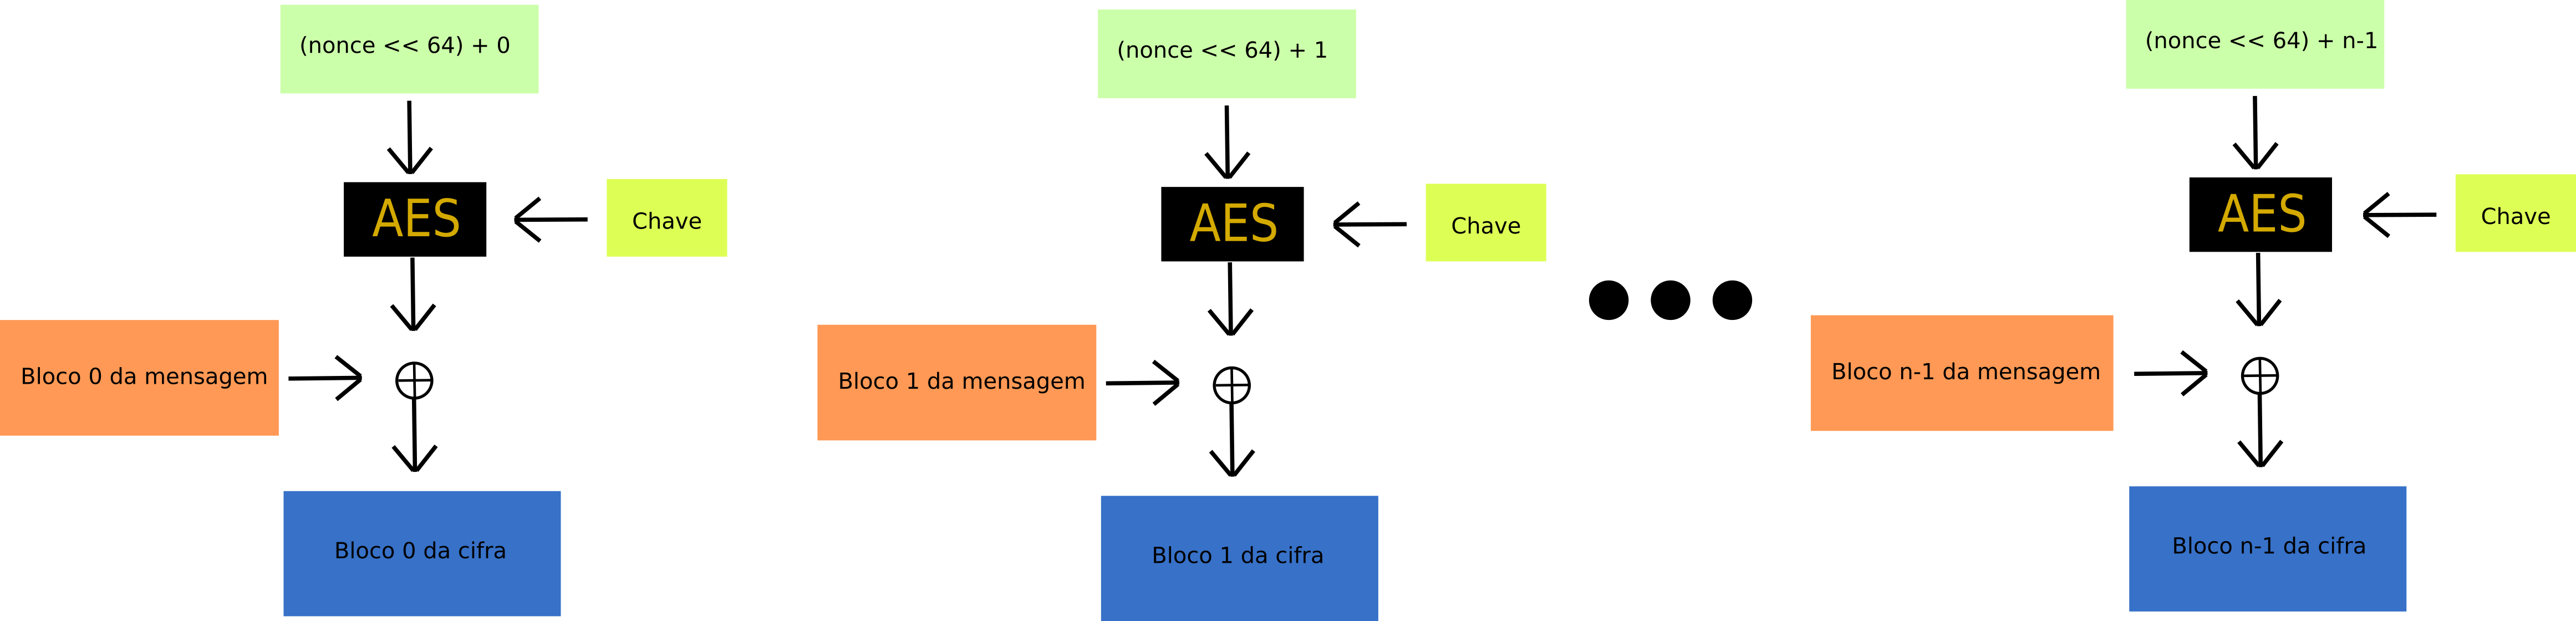
\includegraphics[width=\textwidth]{img/ctr.png}
    \caption{Cifra de bloco no modo CTR}
\end{figure}

Como podemos ver, a mensagem só entra após todo o processo do AES for concluído, onde é feito um XOR entre o output e a mensagem e esta é a nossa cifra. Por este motivo, para reverter a operação, basta realizá-la novamente, pois o inverso de um XOR é o próprio XOR.

\section{Testes}
Para os testes propostos, foi utilizado o formato de imagem PPM, pois é um formato não compactado que contém um header simples com o nível de compactação na primeira linha, a largura e altura na segunda, a profundidade de cores na terceira e no restante do arquivo, os valores RGB para cada pixel. Por ser um formato que tem o valor específico da cor para cada pixel, é um formato ideal para os testes propostos, em especial no modo de compactação \texttt{P6}, que foi o utilizado no projeto.

Foi criada uma classe \texttt{Ppm} que identifica se o arquivo é um PPM P6 válido verificando o seu header. Em caso positivo, o header é separado do resto da mensagem para que não seja cifrado e ao final de todo o processo, o header é adicionado ao criptograma. Com isso, seguem os resultados que podem ser encontrados na pasta \texttt{docs/img} tanto no formato PPM quanto no formato JPG após conversão:

\begin{figure}[H]
	\centering
    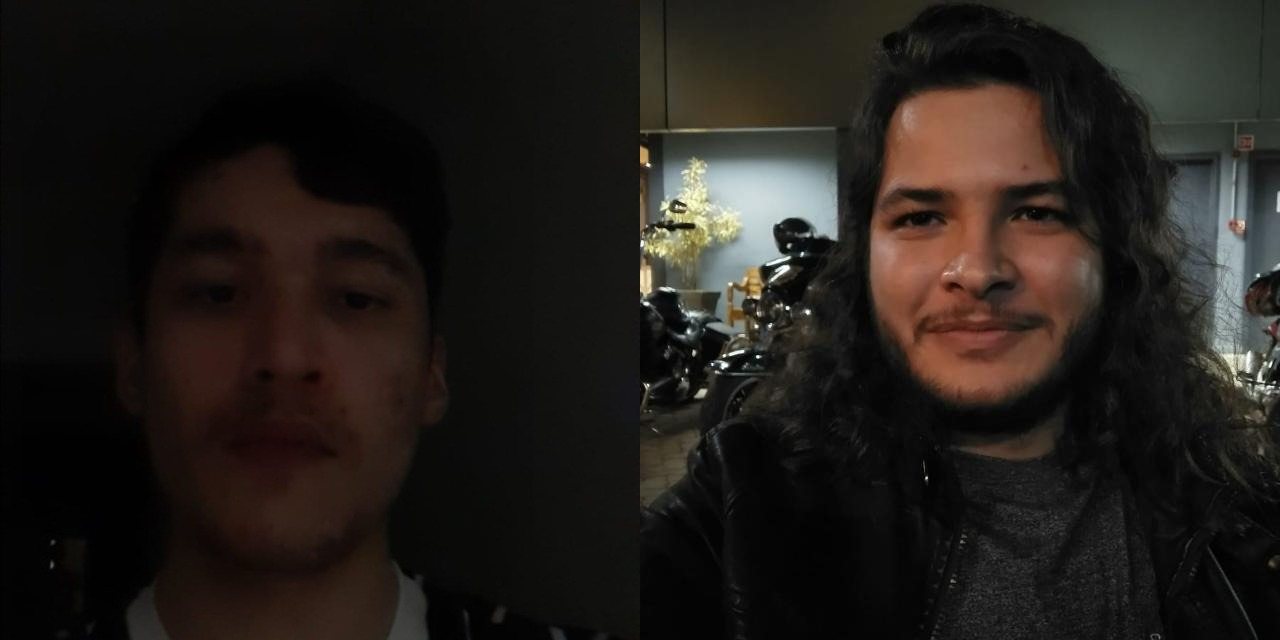
\includegraphics[width=.5\textwidth]{../sample/dupla.jpg}
    \caption{Imagem original (selfie da dupla)}
\end{figure}

A imagem pode ser encontrada na pasta \texttt{sample} tanto no formato PPM quanto no JPG. Os \textit{Hashes} foram gerados com a função MD5 a partir de sua versão PPM e podem ser encontrados abaixo de cada imagem.

\subsection{ECB}

Seguem os testes para o modo ECB usando a chave \texttt{keys/key\_sample} incluindo o comando usado para gerá-los:

\subsubsection{1 Rodada}

\texttt{python src/aes.py sample/dupla.ppm -o docs/img/ecb1.ppm -k keys/key\_sample -r 1}

\begin{figure}[H]
	\centering
    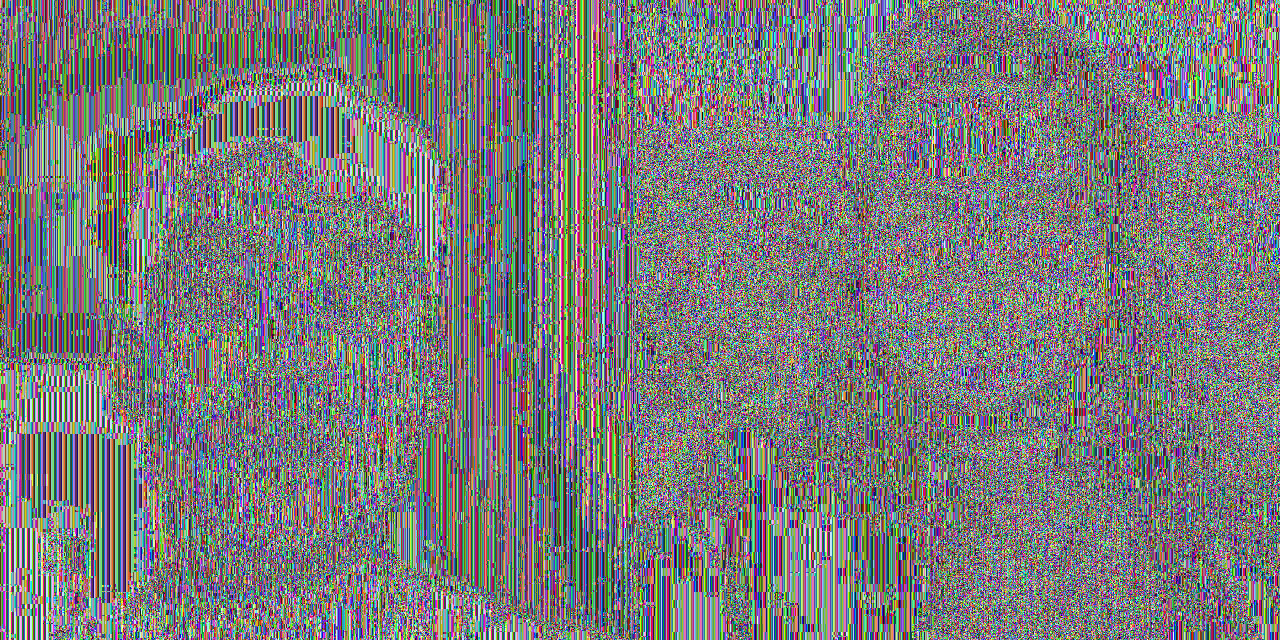
\includegraphics[width=.5\textwidth]{img/ecb1.jpg}
    \caption{Imagem cifrada com 1 rodada do AES}
\end{figure}

\noindent \texttt{MD5 (ecb1.ppm) = 023d6decf1ebb85563fae1668c48c160}

\subsubsection{5 Rodadas}

\texttt{python src/aes.py sample/dupla.ppm -o docs/img/ecb5.ppm -k keys/key\_sample -r 5}

\begin{figure}[H]
	\centering
    
\includegraphics[width=.5\textwidth]{img/ecb5.jpg}
    \caption{Imagem cifrada com 5 rodadas do AES}
\end{figure}

\noindent \texttt{MD5 (ecb5.ppm) = 50f397efc5fd9534c2cccc810b4fbfe8}

\subsubsection{9 Rodadas}

\texttt{python src/aes.py sample/dupla.ppm -o docs/img/ecb9.ppm -k keys/key\_sample -r 9}

\begin{figure}[H]
	\centering
    
\includegraphics[width=.5\textwidth]{img/ecb9.jpg}
    \caption{Imagem cifrada com 9 rodadas do AES}
\end{figure}

\noindent \texttt{MD5 (ecb9.ppm) = 42536ed747de4d4fb1fdf454cfe8006f}

\subsubsection{13 Rodadas}

\texttt{python src/aes.py sample/dupla.ppm -o docs/img/ecb13.ppm -k keys/key\_sample -r 13}

\begin{figure}[H]
	\centering
    
\includegraphics[width=.5\textwidth]{img/ecb13.jpg}
    \caption{Imagem cifrada com 13 rodadas do AES}
\end{figure}

\noindent \texttt{MD5 (ecb13.ppm) = d019478b1d9e122a35cc6146b1985456}

\subsection{Modo CTR}

Seguem os testes para o modo CTR usando a chave \texttt{keys/key\_sample}:

\subsubsection{1 Rodada}

\texttt{python src/aes.py sample/dupla.ppm -o docs/img/ctr1.ppm -k keys/key\_sample -r 1 -m ctr}

\begin{figure}[H]
	\centering
    
\includegraphics[width=.5\textwidth]{img/ctr1.jpg}
    \caption{Imagem cifrada com 1 rodada do AES}
\end{figure}

\noindent \texttt{MD5 (ctr1.ppm) = d477b734b15d441ef5e6675914b30a13}

\subsubsection{5 Rodadas}

\texttt{python src/aes.py sample/dupla.ppm -o docs/img/ctr5.ppm -k keys/key\_sample -r 5 -m ctr}

\begin{figure}[H]
	\centering
    
\includegraphics[width=.5\textwidth]{img/ctr5.jpg}
    \caption{Imagem cifrada com 5 rodadas do AES}
\end{figure}

\noindent \texttt{MD5 (ctr5.ppm) = b28b7012c992e3c354025d0f89dc2163}

\subsubsection{9 Rodadas}

\texttt{python src/aes.py sample/dupla.ppm -o docs/img/ctr9.ppm -k keys/key\_sample -r 9 -m ctr}

\begin{figure}[H]
	\centering
    
\includegraphics[width=.5\textwidth]{img/ctr9.jpg}
    \caption{Imagem cifrada com 9 rodadas do AES}
\end{figure}

\noindent \texttt{MD5 (ctr9.ppm) = 3cfcaac02cfaaebb8ae9dd68e530da01}

\subsubsection{13 Rodadas}

\texttt{python src/aes.py sample/dupla.ppm -o docs/img/ctr13.ppm -k keys/key\_sample -r 13 -m ctr}

\begin{figure}[H]
	\centering
    
\includegraphics[width=.5\textwidth]{img/ctr13.jpg}
    \caption{Imagem cifrada com 13 rodadas do AES}
\end{figure}

\noindent \texttt{MD5 (ctr13.ppm) = 4a89bf7591e1856795057a22cdfa1ec0}

\subsection{Considerações}
Podemos ver que os outputs do ECB contém elementos identificáveis da imagem, mesmo com uma quantidade maior de rodadas, portanto, pode-se considerar que ele é menos seguro que o CTR, que com apenas 1 round ainda mostrou elementos da imagem facilmente reconhecíveis, como um rosto, mas com quantidades de rodadas acima disso, já é impossível reconhecer qualquer elemento da imagem.

\end{document}
